\documentclass[11pt]{article}

\usepackage{amsmath}
\usepackage{amsthm}
\usepackage{amssymb}
\usepackage[textwidth=16cm,textheight=21cm]{geometry}
\usepackage{xcolor}
\usepackage{graphicx}
\usepackage{booktabs}
\usepackage{listings}
\usepackage{hyperref}

% Draft only: line numbers and labels (remove before submission)
\usepackage[mathlines]{lineno}
\renewcommand\linenumberfont{\normalfont\small\color{gray}}
\linenumbers
\usepackage{showlabels}

\lstset{basicstyle=\ttfamily\footnotesize,frame=single,columns=fullflexible,language=Fortran}

\newcommand{\R}{\mathbb{R}}
\newcommand{\UB}{\mathrm{UB}}
\newcommand{\scheme}{TOPBEE-$\delta$}
\newcommand{\todo}[1]{\textcolor{red}{[TODO: #1]}}

\theoremstyle{plain}
\newtheorem{theorem}{Theorem}[section]
\newtheorem{lemma}[theorem]{Lemma}
\newtheorem{proposition}[theorem]{Proposition}
\newtheorem{corollary}[theorem]{Corollary}
\theoremstyle{definition}
\newtheorem{definition}[theorem]{Definition}
\newtheorem{example}[theorem]{Example}
\newtheorem{remark}[theorem]{Remark}

\begin{document}

\title{\scheme: a sensor-blended, CFL-dependent hybrid flux limiter for wave-propagation finite volume schemes}

\author{
    Gustavo Quintero\thanks{Department of Mathematics, Universidad del Atl\'antico, Puerto Colombia, Atl\'antico, Colombia. email: gdquintero@mail.uniatlantico.edu.co}
    \todo{co-authors}
}

\date{\today}
\maketitle

\begin{abstract}
We revisit a hybrid flux limiter that blends a compressive limiter (MINBEE, the arithmetic mean of Superbee and Minmod in the normalized variable diagram) with the polynomial upwind scheme TOPUS through the algebraic smoothness sensor $\omega(r)=\bigl(2|r|/(1+r^2)\bigr)^2$. We show that this hybrid is total variation diminishing (TVD) but only second-order accurate in smooth monotone regions, because it inherits the slope $\Psi'(1)=1/4$ of TOPUS. The key observation is that the sensor satisfies $1-\omega(r)=O\bigl((r-1)^2\bigr)$: any blend driven by it reproduces the smooth component exactly up to $O(|r-1|^3)$. We exploit this property to build \scheme, a one-parameter family $\Psi=(1-\omega_\delta)\,\mathrm{CS}+\omega_\delta\,\mathrm{AR}$ that blends the CFL-Superbee and Arora--Roe limiters with a thresholded sensor $\omega_\delta$, where $\delta=1$ recovers the original sensor. For every $\delta>0$ and every Courant number the family satisfies the CFL-dependent TVD condition and the inclusion property, and is tangent to Roe's third-order scheme at $r=1$; the parameter $\delta$ orders the family monotonically in compressivity. A von Neumann analysis confirms third order near smooth states for every Courant number, whereas the original hybrid is second order and MINBEE is third order only at $\nu=1/2$. The limiter was implemented in the Fortran kernels of CLAWPACK with local Courant numbers per wave. In the one-dimensional Euler tests, every reference configuration considered, including the two configurations recommended by Kemm (2011), is outperformed in both an aggregate shock-test error and a smooth-flow error by some member of the family; in linear advection the same holds for all references except the pure Arora--Roe limiter on smooth data, which is the limit $\delta\to\infty$ of the family. In two dimensions \scheme{} is competitive with Kemm's configurations and clearly superior to MC and to the original hybrid.

\medskip
\noindent
\textbf{Keywords:} Flux limiter, TVD schemes, wave-propagation algorithm, CLAWPACK, third-order tangency,
smoothness sensor, Euler equations.

\medskip
\noindent
\textbf{Mathematics Subject Classification:} 65M08, 65M12, 35L65, 76M12, 76N15.
\end{abstract}

%=====================================================================
\section{Introduction}\label{sec:intro}
High-resolution finite volume schemes for hyperbolic conservation laws combine a second- or higher-order correction with a nonlinear limiter that prevents spurious oscillations near discontinuities \cite{Harten1983,Sweby1984,LeVeque2002}. In the flux-limiter framework the limiter is a function $\Psi(r)$ of the ratio $r$ of consecutive jumps, and Sweby's diagram characterizes the TVD limiters for all Courant numbers $\nu\le 1$. Two lines of work have refined this classical picture.

The first line, initiated by Roe \cite{Roe1986} and Arora and Roe \cite{AroraRoe1997} and systematized by Kemm \cite{Kemm2011}, exploits the fact that the one-step (Lax--Wendroff type) correction used by the wave-propagation algorithms of CLAWPACK \cite{LeVeque1997,LeVeque2002,Clawpack} admits a TVD region that depends on the local Courant number $\nu$ and is much larger than Sweby's region. Limiters that use this freedom---such as CFL-Superbee (Roe's Ultrabee) or the Arora--Roe limiter, which follows Roe's third-order linear scheme near $r=1$---considerably reduce numerical diffusion \cite{Kemm2011}.

The second line, rooted in Leonard's normalized variable diagram (NVD) \cite{Leonard1988} and the convection boundedness criterion \cite{GaskellLau1988}, builds upwind schemes from piecewise polynomial curves in normalized variables. A representative of the Brazilian school is TOPUS \cite{Ferreira2012}, followed by several polynomial and B\'ezier-based variants \cite{CaroCandezano2012,Oviedo2023}. These schemes are usually designed and tested in a semi-discrete setting and are CFL-independent.

This work starts from a hybrid limiter that combines both worlds in a simple way: a compressive, piecewise linear limiter (MINBEE, obtained as the arithmetic mean of Superbee and Minmod in the NVD) is blended with TOPUS through the smoothness sensor $\omega(r)=\bigl(2|r|/(1+r^2)\bigr)^2$, which equals one at $r=1$ and decays for $r\to0$ and $r\to\infty$ \todo{cite the authors' previous note/report on MINBEE and the hybrid, if any}. We analyse this hybrid and identify both its strength and its weakness. The weakness is that the hybrid inherits from TOPUS the slope $\Psi'(1)=1/4$, which makes it second-order accurate for every Courant number. The strength lies in the sensor: since $1-\omega(r)=O((r-1)^2)$, the blend reproduces the smooth component \emph{exactly} up to third-order terms in $r-1$, whatever the compressive component is. This turns the sensor into a device to combine a compressive limiter with a third-order one without losing the tangency to the third-order scheme.

Our contributions are the following.
\begin{itemize}
\item An analysis of the original MINBEE--TOPUS hybrid: TVD property, slope at $r=1$, and the identification of MINBEE with known limiters (Section~\ref{sec:original}).
\item A general order-inheritance theorem for sensor-driven blends and the thresholded sensor $\omega_\delta$, with explicit bounds (Section~\ref{sec:family}).
\item The \scheme{} family: TVD in the CFL-dependent sense, inclusion, third-order tangency for every $\delta$ and monotone ordering in $\delta$; a von Neumann analysis of the resulting schemes near smooth states (Sections~\ref{sec:family}--\ref{sec:vn}).
\item An implementation in the Fortran kernels of CLAWPACK with local Courant numbers, and a systematic comparison with the CFL-dependent limiters of \cite{Kemm2011} on linear advection and the Euler equations in one and two space dimensions (Sections~\ref{sec:impl}--\ref{sec:results}).
\end{itemize}

The rest of this work is organized as follows. Section~\ref{sec:background} recalls the wave-propagation scheme, the TVD conditions and the
ingredients of the original hybrid. Section~\ref{sec:original} analyses the original hybrid. Section~\ref{sec:family} introduces
sensor-driven blends and the \scheme{} family, and Section~\ref{sec:vn} presents the linear analysis near smooth states.
Section~\ref{sec:impl} describes the implementation in CLAWPACK, Section~\ref{sec:results} the numerical results,
Section~\ref{sec:discussion} discusses the results and their limitations, and Section~\ref{sec:conclusions} concludes.

%=====================================================================
\section{Background}\label{sec:background}
\subsection{One-step wave-propagation scheme}
For the linear advection equation $q_t+aq_x=0$ with $a>0$ and Courant number $\nu=a\Delta t/\Delta x\in(0,1]$, the flux-limited one-step scheme reads
\begin{equation}\label{eq:scheme}
Q_i^{n+1}=Q_i^n-\nu\,(Q_i^n-Q_{i-1}^n)-\frac{\nu(1-\nu)}{2}\Bigl[\Psi(r_{i+1/2})\,\Delta Q_{i+1/2}-\Psi(r_{i-1/2})\,\Delta Q_{i-1/2}\Bigr],
\end{equation}
with $\Delta Q_{i+1/2}=Q_{i+1}^n-Q_i^n$ and $r_{i+1/2}=\Delta Q_{i-1/2}/\Delta Q_{i+1/2}$. The choices $\Psi\equiv0$, $\Psi\equiv1$ and $\Psi(r)=r$ give the upwind, Lax--Wendroff and Beam--Warming schemes. For systems, the wave-propagation algorithm \cite{LeVeque1997,LeVeque2002} decomposes each jump into waves $\mathcal{W}^p_{i-1/2}$ moving with speeds $s^p_{i-1/2}$, and adds the correction fluxes
\begin{equation}\label{eq:wavecorr}
\tilde F_{i-1/2}=\frac12\sum_p |s^p_{i-1/2}|\Bigl(1-\frac{\Delta t}{\Delta x}|s^p_{i-1/2}|\Bigr)\,\Psi\bigl(r^p_{i-1/2},\nu^p_{i-1/2}\bigr)\,\mathcal{W}^p_{i-1/2},
\end{equation}
where $r^p$ is the projection of the upwind wave of the same family onto $\mathcal{W}^p$ and $\nu^p_{i-1/2}=|s^p_{i-1/2}|\Delta t/\Delta x$ is the \emph{local} Courant number of the wave.

\subsection{TVD regions and accuracy conditions}
Sweby's (restricted) TVD region, valid for all $\nu\in[0,1]$, is $\Psi(r)=0$ for $r\le0$ and $0\le\Psi(r)\le\min(2r,2)$ for $r>0$ \cite{Sweby1984}. For scheme~\eqref{eq:scheme} with a fixed $\nu\in(0,1)$, Kemm \cite[eq.~(17)]{Kemm2011} gives the general (CFL-dependent) TVD condition
\begin{equation}\label{eq:tvdgen}
-\frac{2}{1-\nu}\le\frac{\Psi(r)}{r}-\Psi(R)\le\frac{2}{\nu}\qquad\text{for all } r,R.
\end{equation}
We use the upper bound $\UB_\nu(r)=\max\bigl(0,\min(2r/\nu,\,2/(1-\nu))\bigr)$ and the following elementary sufficient condition.

\begin{lemma}\label{lem:pointwise}
If $\Psi(r)=0$ for $r\le0$ and $0\le\Psi(r)\le\UB_\nu(r)$ for $r>0$, then $\Psi$ satisfies~\eqref{eq:tvdgen}.
\end{lemma}
\begin{proof}
For $r>0$, $0\le\Psi(r)/r\le2/\nu$; for $r\le0$ we set $\Psi(r)/r=0$ since $\Psi(r)=0$. For every $R$, $0\le\Psi(R)\le 2/(1-\nu)$. Hence $\Psi(r)/r-\Psi(R)\in[-2/(1-\nu),\,2/\nu]$.
\end{proof}

Consistency with second order requires $\Psi(1)=1$. The inclusion property (M2 in \cite{Kemm2011}) reads $\min(1,r)\le\Psi(r)\le\max(1,r)$ for $r>0$. Roe's third-order linear scheme corresponds to
\begin{equation}\label{eq:phi3}
\Phi_3(r;\nu)=1+\frac{1+\nu}{3}\,(r-1),
\end{equation}
and a limiter is called \emph{tangent to the third-order scheme} if $\Psi(1+\varepsilon)=\Phi_3(1+\varepsilon)+O(\varepsilon^2)$ \cite{Roe1986,AroraRoe1997,Kemm2011}.

\paragraph{Reference limiters.} Besides Minmod, Superbee, van Leer and MC we use the CFL-dependent limiters of \cite{AroraRoe1997,Kemm2011}, with a safety factor $\theta\in(\frac12,1]$:
\begin{align}
\mathrm{AR}_\theta(r;\nu)&=\max\bigl(0,\min(\theta\,\UB_\nu(r),\,\Phi_3(r;\nu))\bigr), \label{eq:AR}\\
\mathrm{CS}_\theta(r;\nu)&=\min\bigl(\theta\,\UB_\nu(r),\,\max(1,r)\bigr)\ \ (r>0),\qquad \mathrm{CS}_\theta(r;\nu)=0\ \ (r\le0), \label{eq:CS}
\end{align}
(Arora--Roe and CFL-Superbee, the latter also known as Ultrabee), and Kemm's $\beta$-limiter \cite[eq.~(43)]{Kemm2011} with $\beta=2/3$. We write AR and CS for $\theta=1$.

\subsection{Normalized variables, MINBEE and TOPUS}
In normalized variables $\tilde\phi=(\phi-\phi_U)/(\phi_D-\phi_U)$ \cite{Leonard1988}, a face value $\tilde\phi_f$ and a limiter are related by
\begin{equation}\label{eq:nvd}
\tilde\phi_f=\tilde\phi_C+\tfrac12\Psi(r)\,(1-\tilde\phi_C),\qquad r=\frac{\tilde\phi_C}{1-\tilde\phi_C}.
\end{equation}
\textbf{MINBEE} is defined in the NVD as the arithmetic mean of the Superbee and Minmod characteristics:
\[
\tilde\phi_f^{\mathrm{MB}}=\begin{cases}1.75\,\tilde\phi_C,& 0\le\tilde\phi_C\le\frac13,\\ \tilde\phi_C+\frac14,&\frac13<\tilde\phi_C\le\frac23,\\ 0.25\,\tilde\phi_C+0.75,&\frac23<\tilde\phi_C\le1,\end{cases}
\]
and first-order upwind outside $[0,1]$. Since~\eqref{eq:nvd} is affine in $\Psi$ for fixed $\tilde\phi_C$, averaging in the NVD is the same as averaging the limiter functions, so that
\begin{equation}\label{eq:minbee}
\Psi_{\mathrm{MB}}(r)=\tfrac12\bigl(\Psi_{\mathrm{SB}}(r)+\Psi_{\mathrm{MM}}(r)\bigr)=\max\Bigl(0,\min\bigl(\tfrac32 r,\ \tfrac{1+r}{2},\ \tfrac32\bigr)\Bigr).
\end{equation}
\begin{remark}\label{rem:minbee}
The function~\eqref{eq:minbee} coincides with the MC limiter in which the bound $\min(2,2r)$ is multiplied by $\theta=3/4$, a variant that goes back to van Leer \cite{vanLeer1977} and is described in \cite[\S3.1.1]{Kemm2011}; equivalently, it is the generalized minmod limiter $\mathrm{minmod}(\vartheta\Delta_-,\frac12(\Delta_-+\Delta_+),\vartheta\Delta_+)$ with $\vartheta=1.5$ used in central schemes \cite{NessyahuTadmor1990,KurganovTadmor2000}. The NVD derivation as the mean of the two edges of the second-order TVD region gives a new interpretation of this limiter. We also note that the name ``MINBEE'' is used in part of the literature for the Minmod limiter itself \todo{check Roe/Toro usage; consider renaming}.
\end{remark}
\textbf{TOPUS} \cite{Ferreira2012} with its recommended parameter $\alpha=2$ corresponds to
\begin{equation}\label{eq:topus}
\Psi_{\mathrm T}(r)=\frac{2r(3r+1)}{(1+r)^3}\quad(r>0),\qquad \Psi_{\mathrm T}(r)=0\quad(r\le0).
\end{equation}
It satisfies $\Psi_{\mathrm T}(1)=1$, $\Psi_{\mathrm T}'(1)=1/4$ and $\Psi_{\mathrm T}(r)\to0$ as $r\to\infty$.

%=====================================================================
\section{The original MINBEE--TOPUS hybrid}\label{sec:original}
The original hybrid is
\begin{equation}\label{eq:H0}
H_0(r)=\bigl(1-\omega(r)\bigr)\,\Psi_{\mathrm{MB}}(r)+\omega(r)\,\Psi_{\mathrm T}(r),\qquad \omega(r)=\Bigl(\frac{2|r|}{1+r^2}\Bigr)^2 .
\end{equation}

\begin{lemma}[properties of the sensor]\label{lem:sensor}
For all real $r$:
(i) $0\le\omega(r)\le1$, with $\omega(r)=1$ iff $|r|=1$ and $\omega(0)=0$, $\omega(r)\to0$ as $|r|\to\infty$;
(ii) $\omega(1/r)=\omega(r)$ for $r\ne0$;
(iii) $1-\omega(r)=\bigl((1-r^2)/(1+r^2)\bigr)^2\le 2(r-1)^2$, and $1-\omega(r)=(r-1)^2+O(|r-1|^3)$ as $r\to1$;
(iv) $\omega=A^2$ with $A(r)=2r/(1+r^2)$, the factor by which the van Albada limiter corrects the arithmetic mean, $\Psi_{\mathrm{Alb}}(r)=\frac{1+r}{2}A(r)$ \cite{vanAlbada1982,Kemm2011}.
\end{lemma}
\begin{proof}
(i), (ii), (iv) are immediate. For (iii), $1-\omega=\frac{(1+r^2)^2-4r^2}{(1+r^2)^2}=\frac{(1-r^2)^2}{(1+r^2)^2}=\frac{(r-1)^2(r+1)^2}{(1+r^2)^2}$, and $(r+1)^2\le2(1+r^2)$ gives the bound $2(r-1)^2/(1+r^2)\le2(r-1)^2$. At $r=1$ the factor $(r+1)^2/(1+r^2)^2$ equals one.
\end{proof}

\begin{proposition}\label{prop:H0}
$H_0$ vanishes for $r\le0$, satisfies Sweby's restricted region $0\le H_0\le\min(2r,2)$ (hence it is TVD for every $\nu\in[0,1]$), $H_0(1)=1$, and $H_0'(1)=\Psi_{\mathrm T}'(1)=1/4$.
\end{proposition}
\begin{proof}
Both components vanish for $r\le0$. $\Psi_{\mathrm{MB}}\le\min(\frac32r,\frac32)$ and $\Psi_{\mathrm T}\le\min(2r,2)$, since $\max_r\Psi_{\mathrm T}<1.06$ and $6r+2\le2(1+r)^3$ for $r\ge0$; a convex combination stays in the region. The slope follows from Theorem~\ref{thm:inherit}(c) below with $C=\Psi_{\mathrm{MB}}$ and $S=\Psi_{\mathrm T}$, both Lipschitz with value one at $r=1$.
\end{proof}
We also verified numerically that $H_0$ satisfies the inclusion property M2. By Proposition~\ref{prop:vn} below, the slope $1/4$ makes the hybrid a second-order scheme for every Courant number: the third-order slope $(1+\nu)/3$ ranges in $[1/3,2/3]$. (In semi-discrete $\kappa$-schemes the slope $1/4$ corresponds to QUICK, $\kappa=1/2$, which is also second order for cell averages; there third order requires $\Psi'(1)=1/3$.) The analysis therefore suggests keeping the sensor and replacing the smooth component by one that is third-order in the framework at hand.

%=====================================================================
\section{Sensor-driven blends and the \scheme{} family}\label{sec:family}
\begin{definition}
For $\delta>0$ the \emph{thresholded sensor} is
\begin{equation}\label{eq:omegadelta}
\omega_\delta(r)=\frac{\delta^2\,\omega(r)}{1-\omega(r)+\delta^2\,\omega(r)},\qquad\text{so that}\qquad 1-\omega_\delta=\frac{1-\omega}{1-\omega+\delta^2\omega}.
\end{equation}
Given two limiters $C$ (compressive) and $S$ (smooth), the blended limiter is $\Psi_\delta=(1-\omega_\delta)\,C+\omega_\delta\,S$.
\end{definition}
Clearly $\omega_1=\omega$, $0\le\omega_\delta\le1$, $\omega_\delta(1)=1$, and $\omega_\delta$ is increasing in $\delta$. Writing $\sigma=|1-r^2|/(1+r^2)\in[0,1]$ (so that $1-\omega=\sigma^2$), the blend gives equal weight to $C$ and $S$ when $\sigma=\delta/\sqrt{1+\delta^2}$, i.e.\ at $|r-1|\approx\delta$ for small $\delta$.

\begin{theorem}[sensor-driven blends]\label{thm:inherit}
Let $\theta\in(0,1]$ and let $C(\cdot;\nu)$, $S(\cdot;\nu)$ vanish for $r\le0$ and satisfy $0\le C,S\le\theta\,\UB_\nu$ for $r>0$. Then, for every $\delta>0$:
\begin{enumerate}
\item[(a)] $\Psi_\delta$ satisfies the general TVD condition~\eqref{eq:tvdgen};
\item[(b)] if $C$ and $S$ satisfy the inclusion property M2, so does $\Psi_\delta$;
\item[(c)] if $C(1)=S(1)=1$ and $C,S$ are Lipschitz on $[\frac12,2]$ with constants $L_C,L_S$, then
\[
|\Psi_\delta(r)-S(r)|\le\frac{25}{8}\,\frac{L_C+L_S}{\delta^2}\,|r-1|^3\qquad (r\in[\tfrac12,2]);
\]
in particular $\Psi_\delta(1)=1$, $\Psi_\delta$ is differentiable at $r=1$ whenever $S$ is (even if $C$ is not), and $\Psi_\delta'(1)=S'(1)$;
\item[(d)] if $C\ge S$ for $r>0$, then $\Psi_\delta(r)$ is nonincreasing in $\delta$, $\Psi_\delta\to C$ as $\delta\to0$ for $r>0$, $r\ne1$, and $\Psi_\delta\to S$ as $\delta\to\infty$ for $r>0$.
\end{enumerate}
\end{theorem}
\begin{proof}
(a) and (b): for each $r$, $\Psi_\delta(r)$ is a convex combination of $C(r)$ and $S(r)$, so $0\le\Psi_\delta\le\theta\UB_\nu\le\UB_\nu$ and $\Psi_\delta=0$ for $r\le0$; apply Lemma~\ref{lem:pointwise}. The inclusion bounds are preserved by convex combinations.
(c): $\Psi_\delta-S=(1-\omega_\delta)(C-S)$. By~\eqref{eq:omegadelta}, $1-\omega_\delta\le(1-\omega)/(\delta^2\omega)$. On $[\frac12,2]$, $\omega\ge\omega(\frac12)=\omega(2)=16/25$ (Lemma~\ref{lem:sensor}(ii) and monotonicity of $\omega$ on $(0,1]$), and $1-\omega\le2(r-1)^2$; hence $1-\omega_\delta\le\frac{25}{8}(r-1)^2/\delta^2$. Finally $|C-S|\le|C-1|+|S-1|\le(L_C+L_S)|r-1|$.
(d): $\partial_\delta\omega_\delta=2\delta\,\omega(1-\omega)/(1-\omega+\delta^2\omega)^2\ge0$ and $\Psi_\delta=C-\omega_\delta(C-S)$. The limits follow from $\omega(r)\in(0,1)$ for $r>0$, $r\ne1$.
\end{proof}

\begin{definition}[\scheme]
For $\delta>0$ and $\theta\in(\frac12,1]$,
\begin{equation}\label{eq:topbee}
T_{\delta,\theta}(r;\nu)=\bigl(1-\omega_\delta(r)\bigr)\,\mathrm{CS}_\theta(r;\nu)+\omega_\delta(r)\,\mathrm{AR}_\theta(r;\nu).
\end{equation}
\end{definition}
The name reflects the two ingredients: the \emph{third-order} scheme (as in TOPUS) and the Super\emph{bee} family; for $\delta=1$ the blend uses exactly the sensor of the original hybrid.

\begin{corollary}\label{cor:topbee}
For all $\delta>0$, $\theta\in(\frac12,1]$ and $\nu\in(0,1)$:
(i) $T_{\delta,\theta}$ satisfies~\eqref{eq:tvdgen} and the inclusion property;
(ii) $T_{\delta,\theta}(1+\varepsilon)=\Phi_3(1+\varepsilon)+O(\varepsilon^3)$; in particular it is tangent to Roe's third-order scheme and $T_{\delta,\theta}'(1)=(1+\nu)/3$;
(iii) $T_{\delta,\theta}$ is nonincreasing in $\delta$ and interpolates between $\mathrm{CS}_\theta$ ($\delta\to0$) and $\mathrm{AR}_\theta$ ($\delta\to\infty$).
\end{corollary}
\begin{proof}
For $r>0$, $\Phi_3(r)=1+s(r-1)$ with $s=(1+\nu)/3\in(\frac13,\frac23)$ lies between $\min(1,r)$ and $\max(1,r)$ and is positive. Since $\theta\UB_\nu(r)\ge\theta\min(2r,2)\ge\min(1,r)$ for $\theta\ge\frac12$, both $\mathrm{AR}_\theta$ and $\mathrm{CS}_\theta$ satisfy M2, are bounded by $\theta\UB_\nu$, and $\mathrm{AR}_\theta\le\mathrm{CS}_\theta$. Near $r=1$, $\theta\UB_\nu\ge2\theta>1$, so $\mathrm{AR}_\theta=\Phi_3$ and $\mathrm{CS}_\theta=\max(1,r)$ there; both are Lipschitz. Apply Theorem~\ref{thm:inherit}.
\end{proof}

\begin{remark}[meaning of $\delta$]
For smooth monotone data, $r_{i+1/2}=1-\Delta x\,q''/q'+O(\Delta x^2)$; for a Fourier mode resolved with $N_\lambda$ cells per wavelength, $|r-1|\approx(2\pi/N_\lambda)|\tan\varphi|$, $\varphi$ being the local phase. Thus the third-order component dominates where $|r-1|\lesssim\delta$, i.e.\ $\delta$ fixes the resolution above which a structure is treated as smooth. Small values of $\delta$ yield sharper discontinuities and preserve under-resolved waves, at the price of a later onset of the asymptotic third-order regime under mesh refinement. The family does \emph{not} satisfy the monotonicity property M5 of \cite{Kemm2011}, a property also violated by van Albada-type limiters.
\end{remark}

%=====================================================================
\section{Linear analysis near smooth states}\label{sec:vn}
In smooth monotone regions $r$ is close to one and $\Psi(r)\approx1+\beta(r-1)$, with $\beta=\Psi'(1)$. Then $\Psi(r_{i+1/2})\Delta Q_{i+1/2}\approx(1-\beta)\Delta Q_{i+1/2}+\beta\Delta Q_{i-1/2}$, and~\eqref{eq:scheme} reduces to a one-parameter family of linear schemes ($\beta=0$: Lax--Wendroff; $\beta=1$: Beam--Warming). Its amplification factor for $Q_j=e^{\mathrm{i}j\xi}$ is
\begin{equation}\label{eq:G}
G(\xi)=1-\nu(1-e^{-\mathrm{i}\xi})-\frac{\nu(1-\nu)}{2}(1-e^{-\mathrm{i}\xi})\Bigl[(1-\beta)(e^{\mathrm{i}\xi}-1)+\beta(1-e^{-\mathrm{i}\xi})\Bigr].
\end{equation}
\begin{proposition}\label{prop:vn}
As $\xi\to0$,
\[
G(\xi)-e^{-\mathrm{i}\nu\xi}=\frac{\mathrm{i}}{6}\,\nu(\nu-1)(3\beta-1-\nu)\,\xi^3+\frac{1}{24}\,\nu(\nu-1)(6\beta-\nu-\nu^2)\,\xi^4+O(\xi^5),
\]
\[
|G(\xi)|^2=1-\frac{\nu(\nu-1)}{4}\bigl(\beta(4\nu-2)-\nu-\nu^2\bigr)\,\xi^4+O(\xi^5).
\]
Hence the scheme is third-order accurate if and only if $\beta=(1+\nu)/3$.
\end{proposition}
The expansions were obtained and checked with a computer algebra system. Consequently: the original hybrid ($\beta=1/4$, $3\beta-1-\nu=-(\nu+\frac14)\neq0$) is second order for every $\nu$; MINBEE and MC (slope $1/2$ of Fromm's scheme) are third order only at $\nu=1/2$; \scheme{} is third order near smooth monotone states for every $\nu$, by Corollary~\ref{cor:topbee}(ii). Figure~\ref{fig:vn} compares the amplification factors and phase speeds of these linear schemes, in the spirit of \cite{Lele1992,Pereira2001}.

\begin{figure}[t]\centering
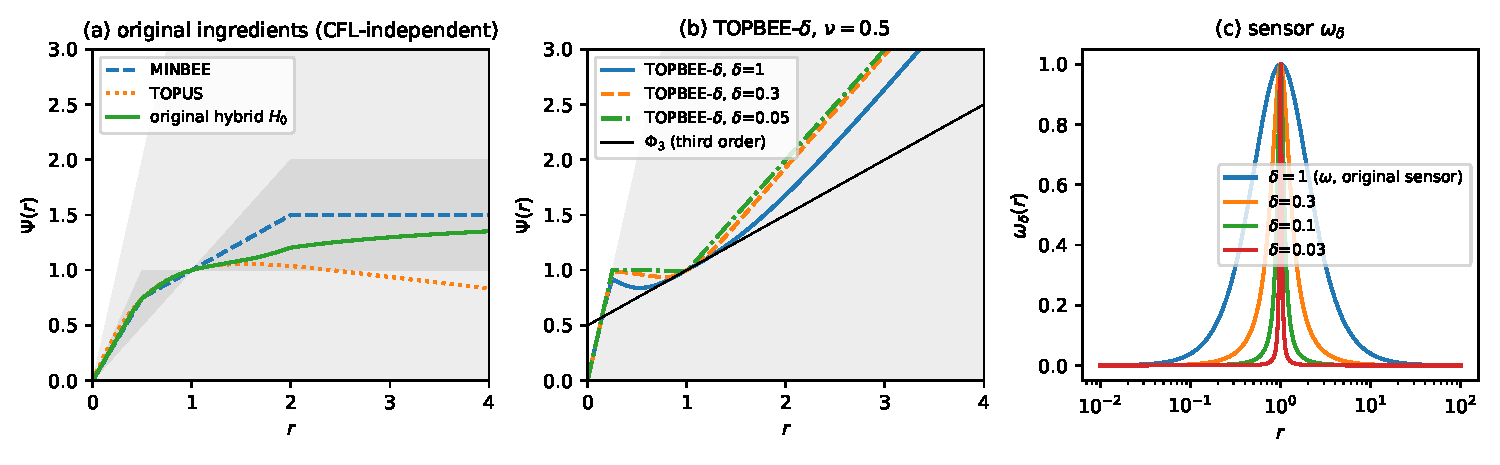
\includegraphics[width=\textwidth]{figures/fig1_limiters.pdf}
\caption{(a) Ingredients of the original hybrid $H_0$ in Sweby's diagram (light grey: TVD region for $\nu=0.5$; dark grey: second-order TVD region). (b) \scheme{} for three values of $\delta$, $\nu=0.5$, $\theta=1$. (c) Thresholded sensor $\omega_\delta$; $\delta=1$ is the original sensor.}\label{fig:lim}
\end{figure}
\begin{figure}[t]\centering
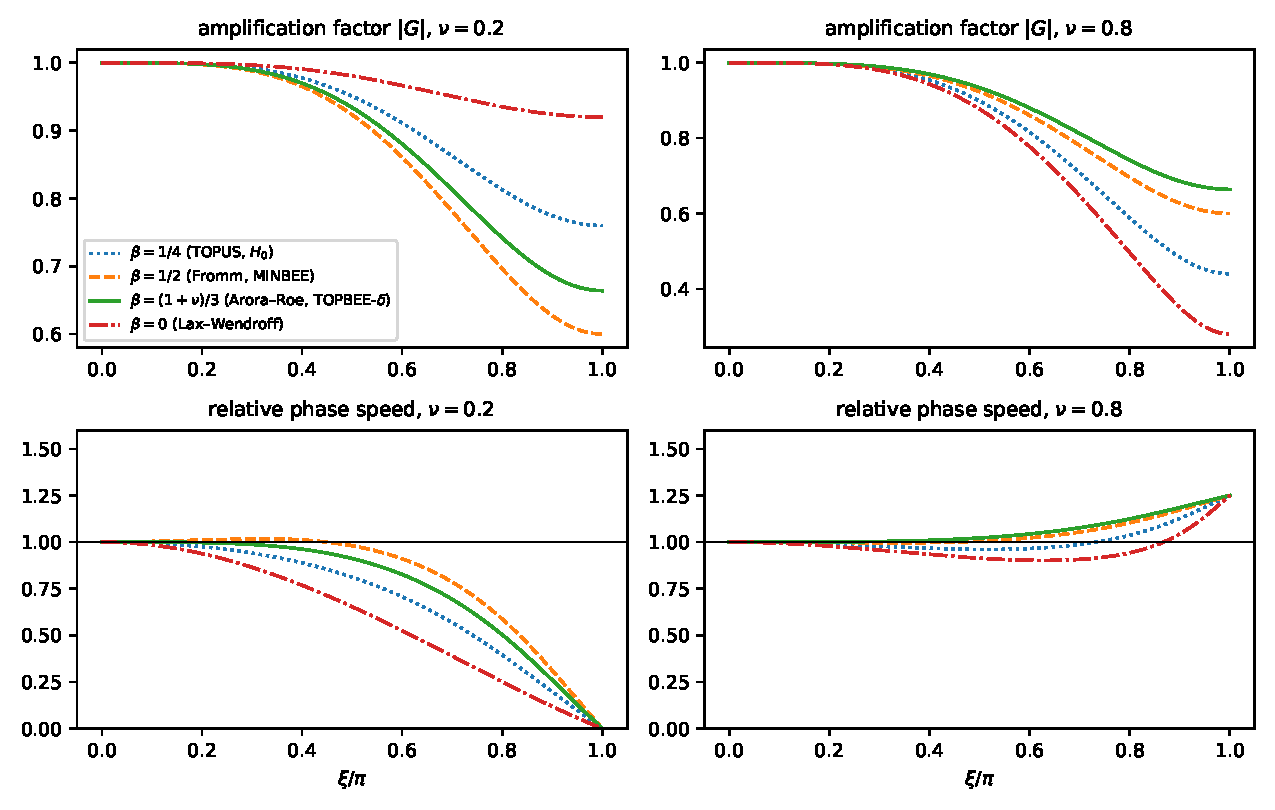
\includegraphics[width=0.85\textwidth]{figures/fig2_vonneumann.pdf}
\caption{Amplification factor and relative phase speed of the linearized schemes near smooth states, $\Psi\approx1+\beta(r-1)$, for $\nu=0.2$ and $\nu=0.8$.}\label{fig:vn}
\end{figure}

%=====================================================================
\section{Implementation in CLAWPACK}\label{sec:impl}
The classic Fortran kernels of CLAWPACK (\texttt{limiter.f90} and \texttt{philim.f90}, used by PyClaw \cite{PyClaw2012} and Clawpack~5 \cite{Clawpack,Mandli2016}) pass only the wave strengths to the limiter function. We added the local Courant number of each wave, computed as in the CFL estimate of \texttt{flux2.f90}:
\[
\nu^p_{i-1/2}=\begin{cases} s^p_{i-1/2}\,(\Delta t/\Delta x)_i,& s^p_{i-1/2}>0,\\ -s^p_{i-1/2}\,(\Delta t/\Delta x)_{i-1},& s^p_{i-1/2}\le0,\end{cases}
\]
which also covers capacity functions. In \texttt{philim} we clip $\nu$ to $[10^{-3},1-10^{-3}]$. The modified kernel reproduces the original kernel bit-for-bit with the MC limiter (the code of the classical limiters is unchanged), and the Fortran implementations of all limiters agree with independent Python implementations to round-off. Listing~\ref{lst:philim} shows the core of the implementation; the extra cost of \scheme{} on a $200\times200$ Euler computation was about 14\% of the total run time compared with MC and 8\% compared with Kemm's mixed configuration.

\paragraph{Systems and choice of parameters.} Following \cite{Kemm2011}, limiters may be chosen per wave family. In all Euler computations we use
\begin{itemize}
\item nonlinear (acoustic) waves: $T_{1,0.75}$, i.e.\ the original sensor ($\delta=1$) with the safety factor $\theta=0.75$;
\item linearly degenerate waves (entropy, shear): $T_{\delta_c,1}$ with $\delta_c\in[0.03,1]$.
\end{itemize}
The safety factor is essential for strong nonlinear waves: in the Woodward--Colella blast wave, every limiter that uses the full CFL-dependent freedom on the acoustic waves (Arora--Roe, CFL-Superbee, Kemm's $\beta$-limiter and \scheme{} with $\theta=1$) produced negative pressures within the first time steps in our computations with the Roe solver, in line with the oscillations reported in \cite[\S5.1]{Kemm2011}, whereas $\theta=0.75$ removed the problem. Bounding $\nu$ from below did not.

%=====================================================================
\section{Numerical results}\label{sec:results}
All computations use the one-step wave-propagation scheme of CLAWPACK~5.14. For linear advection we implemented~\eqref{eq:scheme} directly; the Euler computations use PyClaw with the Roe solver and the Harten--Hyman entropy fix, $\gamma=1.4$, target CFL number $0.9$ (results at CFL $0.5$ are qualitatively identical and omitted) \todo{decide whether to add CFL 0.5 tables}. Errors are $L_1$ norms of cell averages.

\subsection{Linear advection}
We solve $q_t+q_x=0$ on $[-1,1]$ with periodic boundaries, using the Zalesak-type test with four shapes \cite{JiangShu1996} ($N=200$, $t=20$), a wave packet $e^{-50x^2}\sin(20\pi x)$ ($N=200$, $t=10$, about ten cells per wavelength) and $\sin(6\pi x)$ for convergence studies. The number of steps is chosen so that the final time is reached exactly.

Table~\ref{tab:adv} and Figure~\ref{fig:adv} summarize the results. Replacing TOPUS by the Arora--Roe limiter and MINBEE by CFL-Superbee ($\delta=1$) reduces the Zalesak error of the original hybrid by a factor $2.3$--$2.5$ and the smooth error by a factor of about 25, with observed order $2.4$ instead of $2.0$. Decreasing $\delta$ moves the scheme along a trade-off curve (Figure~\ref{fig:adv}a) that lies below all reference limiters except the pure Arora--Roe limiter, which is the limit $\delta\to\infty$ of the family and remains the most accurate one for smooth data. For $\delta=0.03$ the Zalesak error is smaller than that of Kemm's $\beta$-limiter for all three Courant numbers, and for $\delta=0.05$ for $\nu=0.5$ and $0.9$; at $\nu=0.5$ the under-resolved wave packet is preserved four ($\delta=0.05$) to eight ($\delta=0.03$) times better than with the $\beta$-limiter (Figure~\ref{fig:adv}b). On very coarse grids for smooth data (about 17 cells per wavelength) the $\beta$-limiter is about 20\% more accurate. For small $\delta$ the asymptotic order is reached only on finer grids (Figure~\ref{fig:adv}c), as anticipated by the remark on the meaning of $\delta$.

\begin{table}[t]\centering\footnotesize\setlength{\tabcolsep}{3.5pt}
\caption{Linear advection with the one-step wave-propagation scheme: $L_1$ errors. Zalesak test ($N=200$, $t=20$) for three Courant numbers; wave packet ($N=200$, $t=10$, $\nu=0.5$); $\sin 6\pi x$ after one period ($\nu=0.9$, $N=3200$) and observed order between $N=800$ and $N=3200$.}\label{tab:adv}
\begin{tabular}{lcccccc}\toprule
 & \multicolumn{3}{c}{Zalesak} & wave packet & \multicolumn{2}{c}{$\sin 6\pi x$, $\nu=0.9$} \\ \cmidrule(lr){2-4}\cmidrule(lr){6-7}
limiter & $\nu=0.1$ & $\nu=0.5$ & $\nu=0.9$ & $\nu=0.5$ & $N=3200$ & order \\ \midrule
MINBEE & $2.87\mathrm{e}{-1}$ & $1.92\mathrm{e}{-1}$ & $1.15\mathrm{e}{-1}$ & $1.60\mathrm{e}{-1}$ & $1.18\mathrm{e}{-4}$ & 2.09 \\
MC & $2.66\mathrm{e}{-1}$ & $1.67\mathrm{e}{-1}$ & $1.05\mathrm{e}{-1}$ & $1.60\mathrm{e}{-1}$ & $9.91\mathrm{e}{-5}$ & 2.02 \\
$H_0$ (original hybrid) & $3.53\mathrm{e}{-1}$ & $3.14\mathrm{e}{-1}$ & $1.70\mathrm{e}{-1}$ & $1.60\mathrm{e}{-1}$ & $3.03\mathrm{e}{-4}$ & 1.97 \\
Arora--Roe & $1.83\mathrm{e}{-1}$ & $1.51\mathrm{e}{-1}$ & $8.10\mathrm{e}{-2}$ & $1.59\mathrm{e}{-1}$ & $5.29\mathrm{e}{-6}$ & 2.52 \\
CFL-Superbee & $7.52\mathrm{e}{-2}$ & $3.05\mathrm{e}{-2}$ & $3.45\mathrm{e}{-2}$ & $5.18\mathrm{e}{-3}$ & $3.22\mathrm{e}{-4}$ & 1.92 \\
Kemm $\beta=2/3$ & $4.67\mathrm{e}{-2}$ & $5.02\mathrm{e}{-2}$ & $3.94\mathrm{e}{-2}$ & $1.04\mathrm{e}{-1}$ & $2.17\mathrm{e}{-4}$ & 1.94 \\
TOPBEE-$\delta$, $\delta=1$ & $1.55\mathrm{e}{-1}$ & $1.29\mathrm{e}{-1}$ & $6.72\mathrm{e}{-2}$ & $1.56\mathrm{e}{-1}$ & $1.22\mathrm{e}{-5}$ & 2.41 \\
TOPBEE-$\delta$, $\delta=0.3$ & $1.12\mathrm{e}{-1}$ & $9.13\mathrm{e}{-2}$ & $5.12\mathrm{e}{-2}$ & $1.27\mathrm{e}{-1}$ & $4.46\mathrm{e}{-5}$ & 2.32 \\
TOPBEE-$\delta$, $\delta=0.05$ & $5.03\mathrm{e}{-2}$ & $4.30\mathrm{e}{-2}$ & $3.53\mathrm{e}{-2}$ & $2.45\mathrm{e}{-2}$ & $2.08\mathrm{e}{-4}$ & 2.09 \\
TOPBEE-$\delta$, $\delta=0.03$ & $3.63\mathrm{e}{-2}$ & $3.66\mathrm{e}{-2}$ & $3.16\mathrm{e}{-2}$ & $1.27\mathrm{e}{-2}$ & $2.61\mathrm{e}{-4}$ & 2.02 \\
\bottomrule\end{tabular}\end{table}
\begin{table}[t]\centering\footnotesize\setlength{\tabcolsep}{3.5pt}
\caption{Euler equations in 1D (CLAWPACK, Roe solver with Harten--Hyman entropy fix, CFL $0.9$): $L_1$ error of the density. Sod and Lax with $N=200$ (exact solution); Shu--Osher and Woodward--Colella with $N=400$ (reference: $N=12800$); smooth entropy wave with $N=200$ and observed order between $N=400$ and $N=800$. Limiters per wave family: acoustic / contact.}\label{tab:euler1d}
\begin{tabular}{lcccccc}\toprule
scheme (acoustic / contact) & Sod & Lax & Shu--Osher & W--C blast & entropy wave & order \\ \midrule
MC / MC & $1.77\mathrm{e}{-3}$ & $6.34\mathrm{e}{-3}$ & $3.15\mathrm{e}{-1}$ & $9.06\mathrm{e}{-2}$ & $1.22\mathrm{e}{-4}$ & 2.13 \\
Superbee / Superbee & $1.29\mathrm{e}{-3}$ & $4.00\mathrm{e}{-3}$ & $2.11\mathrm{e}{-1}$ & $6.14\mathrm{e}{-2}$ & $6.05\mathrm{e}{-4}$ & 1.97 \\
MINBEE / MINBEE & $1.98\mathrm{e}{-3}$ & $7.05\mathrm{e}{-3}$ & $3.96\mathrm{e}{-1}$ & $9.82\mathrm{e}{-2}$ & $1.95\mathrm{e}{-4}$ & 2.22 \\
$H_0$ / $H_0$ & $2.28\mathrm{e}{-3}$ & $8.04\mathrm{e}{-3}$ & $4.28\mathrm{e}{-1}$ & $1.05\mathrm{e}{-1}$ & $3.97\mathrm{e}{-4}$ & 2.03 \\
AR$_{0.75}$ / AR$_{0.75}$ (Kemm) & $1.67\mathrm{e}{-3}$ & $5.95\mathrm{e}{-3}$ & $2.68\mathrm{e}{-1}$ & $8.39\mathrm{e}{-2}$ & $4.09\mathrm{e}{-5}$ & 2.39 \\
AR$_{0.75}$ / CFL-Superbee (Kemm) & $1.43\mathrm{e}{-3}$ & $2.93\mathrm{e}{-3}$ & $8.21\mathrm{e}{-2}$ & $4.36\mathrm{e}{-2}$ & $5.94\mathrm{e}{-4}$ & 1.96 \\
$T_{1,0.75}$ / $T_{1,1}$ & $1.53\mathrm{e}{-3}$ & $5.01\mathrm{e}{-3}$ & $1.78\mathrm{e}{-1}$ & $7.15\mathrm{e}{-2}$ & $3.41\mathrm{e}{-5}$ & 2.42 \\
$T_{1,0.75}$ / $T_{0.3,1}$ & $1.43\mathrm{e}{-3}$ & $4.09\mathrm{e}{-3}$ & $1.24\mathrm{e}{-1}$ & $5.97\mathrm{e}{-2}$ & $1.18\mathrm{e}{-4}$ & 2.35 \\
$T_{1,0.75}$ / $T_{0.05,1}$ & $1.39\mathrm{e}{-3}$ & $2.95\mathrm{e}{-3}$ & $7.61\mathrm{e}{-2}$ & $4.86\mathrm{e}{-2}$ & $4.54\mathrm{e}{-4}$ & 2.18 \\
$T_{1,0.75}$ / $T_{0.03,1}$ & $1.39\mathrm{e}{-3}$ & $2.84\mathrm{e}{-3}$ & $7.24\mathrm{e}{-2}$ & $4.62\mathrm{e}{-2}$ & $5.31\mathrm{e}{-4}$ & 2.10 \\
\bottomrule\end{tabular}\end{table}
\begin{table}[t]\centering\footnotesize\setlength{\tabcolsep}{3.5pt}
\caption{Euler equations in 2D (CLAWPACK, unsplit with transverse corrections, CFL $0.9$): errors relative to MC (values $<1$ are better than MC). Riemann problem: $L_1$ density error at $200^2$ against an $800^2$ reference computed with MC; implosion: $L_1$ density error against a 1D radial reference; Gresho vortex: $L_1$ velocity error against the exact solution on $4N\times N$ grids. Limiters per wave family: acoustic / (entropy, shear).}\label{tab:euler2d}
\begin{tabular}{lcccccc}\toprule
scheme & Riemann $200^2$ & impl.\ $100^2$ & impl.\ $200^2$ & Gresho $N=20$ & $N=40$ & $N=80$ \\ \midrule
MC & 1.00 & 1.00 & 1.00 & 1.00 & 1.00 & 1.00 \\
Superbee & 1.04 & 0.80 & 0.78 & 1.33 & 3.08 & 0.45 \\
MINBEE & 1.00 & 1.03 & 1.04 & 1.14 & 1.21 & 1.23 \\
$H_0$ & 1.09 & 1.14 & 1.16 & 1.21 & 1.11 & 1.94 \\
AR$_{0.75}$ (Kemm) & 0.97 & 0.99 & 0.98 & 0.94 & 1.01 & 0.78 \\
AR$_{0.75}$ / CFL-Superbee (Kemm) & 1.72 & 0.97 & 0.96 & 0.50 & 0.51 & 0.53 \\
$T_{1,0.75}$ / $T_{1,1}$ & 1.31 & 0.96 & 0.96 & 0.70 & 0.91 & 0.58 \\
$T_{1,0.75}$ / $T_{0.3,1}$ & 1.57 & 0.96 & 0.96 & 0.55 & 0.81 & 0.44 \\
$T_{1,0.75}$ / $T_{0.05,1}$ & 2.01 & 0.95 & 0.95 & 0.51 & 0.69 & 0.48 \\
\bottomrule\end{tabular}\end{table}


\begin{figure}[t]\centering
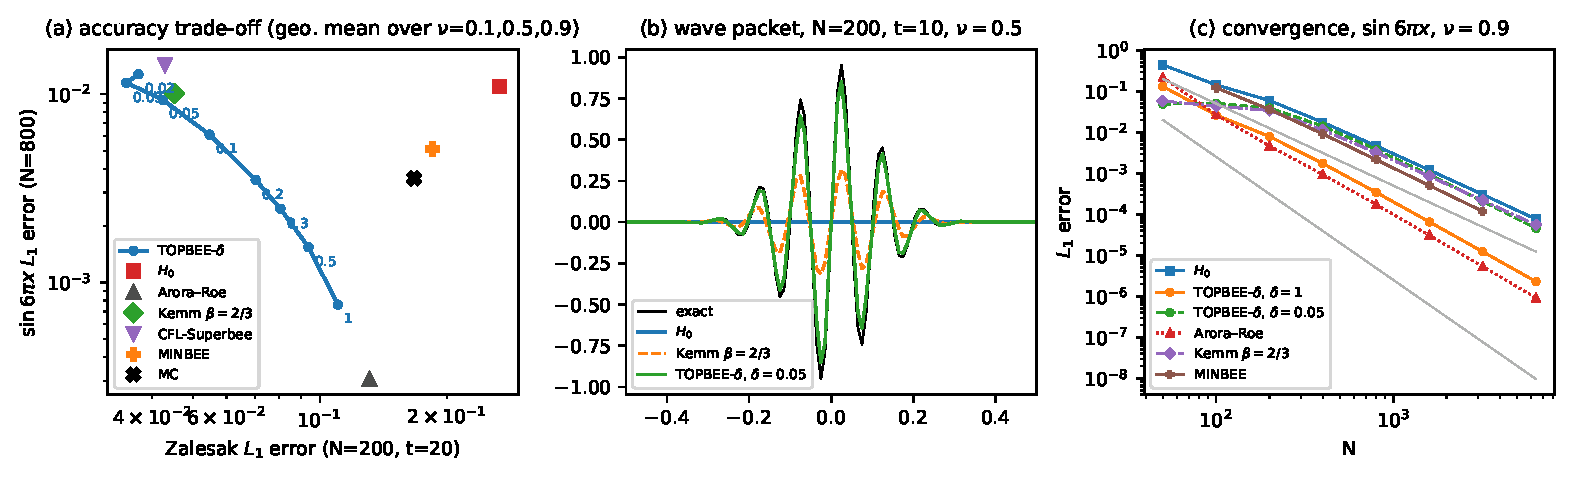
\includegraphics[width=\textwidth]{figures/fig3_advection.pdf}
\caption{Linear advection. (a) Error on discontinuous data versus error on smooth data (geometric mean over $\nu=0.1,0.5,0.9$); numbers label $\delta$. (b) Wave packet. (c) Convergence for $\sin6\pi x$, $\nu=0.9$; grey lines: slopes 2 and 3.}\label{fig:adv}
\end{figure}

\subsection{Euler equations in one dimension}
We consider the Sod and Lax shock tubes ($N=200$, compared with the exact solution), the Shu--Osher shock--entropy interaction \cite{ShuOsher1989} and the Woodward--Colella blast wave \cite{WoodwardColella1984} ($N=400$, reference with $N=12800$ and MC), and a smooth entropy wave $\rho=1+\frac12\sin2\pi x$, $u=p=1$, advected over one period. Table~\ref{tab:euler1d} and Figure~\ref{fig:euler1d} show the results. Every member of the family improves on MC, on MINBEE and on the original hybrid in all shock tests. Varying $\delta_c$ on the contact wave produces a trade-off curve that passes below and to the left of every reference configuration (Figure~\ref{fig:euler1d}a):
\begin{itemize}
\item $\delta_c=1$ is more accurate than Kemm's $\mathrm{AR}_{0.75}$ on all waves in every test, including the smooth one;
\item $\delta_c=0.3$ is more accurate than MC in every test;
\item $\delta_c=0.03$ yields a smaller geometric-mean shock error and a smaller smooth error than Kemm's recommended configuration (CFL-Superbee on the contact, $\mathrm{AR}_{0.75}$ on the acoustic waves), although the latter remains about 6\% better on the blast wave.
\end{itemize}

\begin{figure}[t]\centering
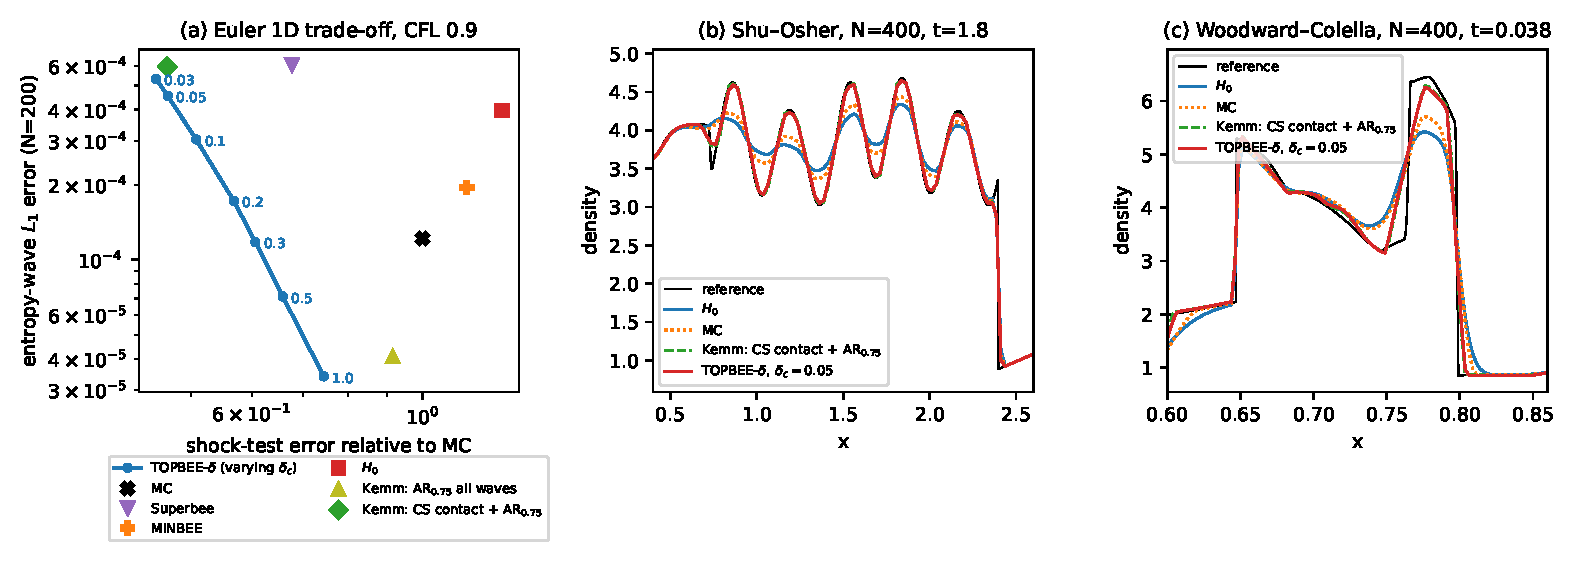
\includegraphics[width=\textwidth]{figures/fig4_euler1d.pdf}
\caption{Euler equations in 1D, CFL $0.9$. (a) Shock-test error (geometric mean of the $L_1$ errors relative to MC over Sod, Lax, Shu--Osher and blast wave) versus smooth entropy-wave error; numbers label $\delta_c$. (b) Shu--Osher problem. (c) Woodward--Colella blast wave.}\label{fig:euler1d}
\end{figure}

\subsection{Euler equations in two dimensions}
We use the unsplit wave-propagation algorithm with transverse corrections and the four-wave Roe solver of CLAWPACK, and the three tests of \cite[\S5.3--5.5]{Kemm2011}: the two-dimensional Riemann problem of \cite{SchulzRinne1993,LiskaWendroff2003} (configuration~3, $200\times200$, $t=0.8$), Toro's implosion problem \cite{Toro2009} on a quarter domain ($t=0.25$, reference from a 1D radial computation with $16000$ cells), and the Gresho vortex \cite{GreshoChan1990} translated with unit speed in $[0,4]\times[0,1]$ ($t=3$). Results are reported in Table~\ref{tab:euler2d} and Figure~\ref{fig:euler2d}.

In two dimensions the picture is less clear-cut than in 1D. For the implosion problem all CFL-dependent configurations perform similarly ($0.95$--$0.99$ of the MC error), with \scheme{} slightly ahead; Superbee is the most accurate here. For the Gresho vortex, \scheme{} with $\delta_c=0.05$ and Kemm's configuration have between $0.48$ and $0.69$ of the error of MC; they are equivalent on the coarsest grid, Kemm's configuration is better on the intermediate grid and \scheme{} on the finest grid. For the Riemann problem the $L_1$ error against a fine-grid reference is not a meaningful measure: the problem is unstable \cite{Kemm2011}, and the less dissipative schemes resolve Kelvin--Helmholtz roll-ups along the slip lines whose position differs from that of the reference; all configurations that are compressive on the linear waves, including Kemm's, have a larger $L_1$ error than MC. Visually (Figure~\ref{fig:euler2d}a--d) both Kemm's configuration and \scheme{} reveal much more structure than MC and the original hybrid. Overall, in 2D \scheme{} is competitive with the best configuration of \cite{Kemm2011}, but does not dominate it.

\begin{figure}[t]\centering
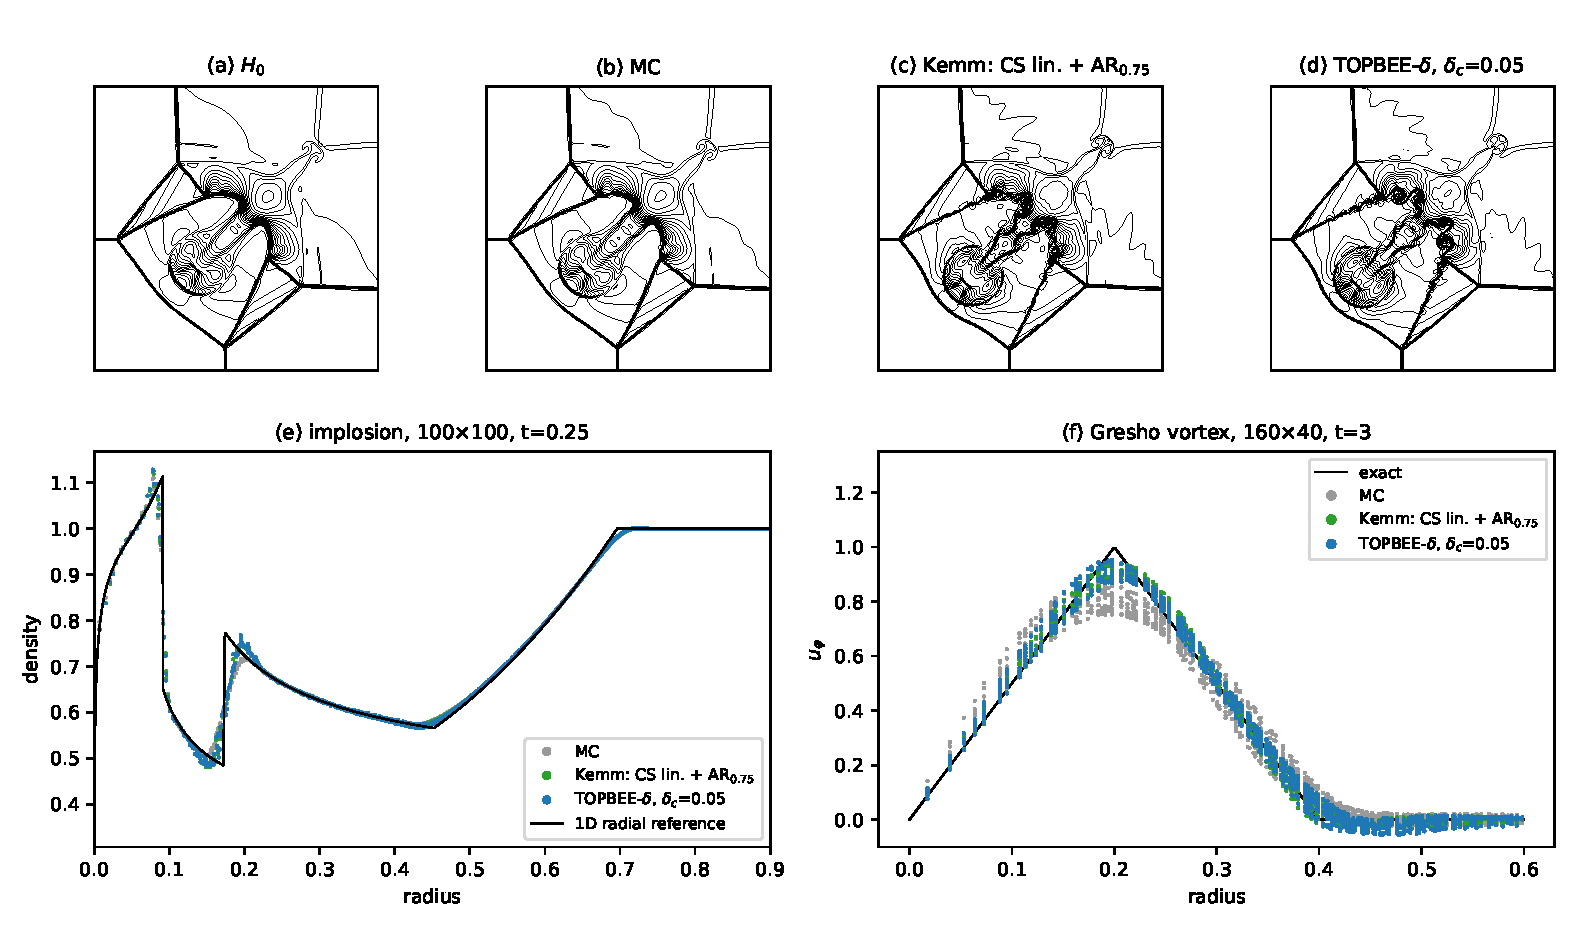
\includegraphics[width=\textwidth]{figures/fig5_euler2d.pdf}
\caption{Euler equations in 2D. (a)--(d) Density contours (30 levels) for the Riemann problem, $200\times200$. (e) Implosion: density versus radius, $100\times100$. (f) Gresho vortex: azimuthal velocity versus radius, $160\times40$.}\label{fig:euler2d}
\end{figure}

%=====================================================================
\section{Discussion}\label{sec:discussion}
\paragraph{What the sensor brings.} The essential property of the sensor $\omega$ is the quadratic contact $1-\omega=O((r-1)^2)$ at $r=1$, combined with $\omega\to0$ for $r\to0$ and $r\to\infty$. Any compressive limiter can be added to a third-order limiter through this sensor without destroying the tangency to the third-order scheme; the deviation from the smooth component is $O(|r-1|^3)$ and the blend removes the kink of CFL-Superbee at $r=1$. Kemm \cite[eqs.~(44)--(45)]{Kemm2011} proposes blending limiters with Harten's switch $\eta=|1-r|/(1+|r|)$, which vanishes linearly at $r=1$; a blend of Arora--Roe and CFL-Superbee with $\eta$ is also tangent, with a deviation $O(|r-1|^2)$, but Kemm uses the switch only to vary $\beta$ in the $\beta$-limiter, which is not tangent at $r=1$. What matters in practice is (i) a weight that vanishes at least linearly at $r=1$ and (ii) a threshold controlling the width of the smooth window; in preliminary tests a thresholded Harten switch gave results similar to $\omega_\delta$ \todo{quantify, or drop}. The sensor $\omega$ of the original hybrid has the advantages of quadratic contact, symmetry $\omega(1/r)=\omega(r)$, a closed-form one-parameter extension and the direct link with the van Albada limiter.

\paragraph{Choice of $\delta$.} We recommend $\delta=1$ (the original sensor) with $\theta=0.75$ on nonlinear waves, and $\delta_c\in[0.03,0.3]$ on linearly degenerate waves: small values for flows dominated by contact discontinuities and under-resolved waves, larger values when smooth structures dominate.

\paragraph{Limitations.} The family violates the monotonicity property M5; the asymptotic third order appears late under refinement for small $\delta$; in 2D the gains with respect to the best existing CFL-dependent configurations are not systematic; and, like all limiters discussed here, \scheme{} is designed for the one-step scheme. A semi-discrete counterpart, in which the smooth component would follow the slope $1/3$ of the $\kappa=1/3$ scheme, is a natural extension, as are an adaptive choice of $\delta$ and tests with adaptive mesh refinement.

%=====================================================================
\section{Conclusions}\label{sec:conclusions}
Starting from a hybrid of MINBEE and TOPUS driven by the sensor $\omega=(2|r|/(1+r^2))^2$, we showed that the sensor guarantees exact inheritance of the smooth component near $r=1$, and used it to build \scheme, a one-parameter family of CFL-dependent limiters for the wave-propagation algorithm. Every member is TVD in the CFL-dependent sense, satisfies the inclusion property and is tangent to Roe's third-order scheme; the parameter $\delta$ orders the family in compressivity, and $\delta=1$ uses exactly the original sensor. Implemented in CLAWPACK with local Courant numbers, the family improves substantially on the original hybrid in all tests, matches or improves on the best configurations of \cite{Kemm2011} in linear advection and one-dimensional gas dynamics, and is competitive with them in two dimensions.

\paragraph{Code availability.} \todo{repository with the modified CLAWPACK kernels, limiter library and scripts}

\paragraph{Acknowledgements.} \todo{funding}. \todo{Disclose the use of AI-assisted tools according to the journal's policy.}

%=====================================================================
\appendix
\section{Fortran implementation}\label{app:code}
\begin{lstlisting}[caption={Core of the modified \texttt{philim.f90} (TOPBEE branch). \texttt{csf}, \texttt{arf} evaluate~\eqref{eq:CS} and~\eqref{eq:AR}; \texttt{omf} evaluates $\omega$.},label={lst:philim}]
double precision function philim(a,b,meth,cfl)
  implicit double precision (a-h,o-z)
  common /limpar/ hdelta(20), htheta(20)
  r = b/a
  select case (meth)
  ...
  case (101:120)                       ! TOPBEE-delta
     k  = meth - 100
     w  = omf(r)                       ! (2|r|/(1+r^2))^2
     d2 = hdelta(k)**2
     w  = d2*w / (1.d0 - w + d2*w)     ! thresholded sensor
     philim = (1.d0-w)*csf(r,cfl,htheta(k)) + w*arf(r,cfl,htheta(k))
  ...
  end select
end function philim
\end{lstlisting}

\clearpage

\begin{thebibliography}{99}

\bibitem{AroraRoe1997} M. Arora and P. L. Roe, A well-behaved TVD limiter for high-resolution calculations of unsteady flow, \textit{Journal of Computational Physics} 132, pp. 3--11, 1997.

% TODO: verify bibliographic data
\bibitem{CaroCandezano2012} M. A. Caro Candezano, \textit{Desenvolvimento de esquema upwind para equa\c{c}\~oes de conserva\c{c}\~ao e implementa\c{c}\~ao de modelagens URANS com aplica\c{c}\~ao em escoamentos incompress\'{\i}veis}, PhD thesis, ICMC-USP, S\~ao Carlos, 2012.

\bibitem{Clawpack} Clawpack Development Team, Clawpack software, version 5.14, \todo{Zenodo DOI}.

\bibitem{Ferreira2012} V. G. Ferreira, R. A. B. Queiroz, G. A. B. Lima, R. G. Cuenca, C. M. Oishi, J. L. F. Azevedo, and S. McKee, A bounded upwinding scheme for computing convection-dominated transport problems, \textit{Computers \& Fluids} 57, pp. 208--224, 2012.

\bibitem{GaskellLau1988} P. H. Gaskell and A. K. C. Lau, Curvature-compensated convective transport: SMART, a new boundedness-preserving transport algorithm, \textit{International Journal for Numerical Methods in Fluids} 8, pp. 617--641, 1988.

% TODO: verify bibliographic data
\bibitem{GreshoChan1990} P. M. Gresho and S. T. Chan, On the theory of semi-implicit projection methods for viscous incompressible flow and its implementation via a finite element method that also introduces a nearly consistent mass matrix. Part 2: Implementation, \textit{International Journal for Numerical Methods in Fluids} 11, pp. 621--659, 1990.

\bibitem{Harten1983} A. Harten, High resolution schemes for hyperbolic conservation laws, \textit{Journal of Computational Physics} 49, pp. 357--393, 1983.

\bibitem{JiangShu1996} G.-S. Jiang and C.-W. Shu, Efficient implementation of weighted ENO schemes, \textit{Journal of Computational Physics} 126, pp. 202--228, 1996.

\bibitem{Kemm2011} F. Kemm, A comparative study of TVD-limiters---well-known limiters and an introduction of new ones, \textit{International Journal for Numerical Methods in Fluids} 67, pp. 404--440, 2011.

\bibitem{PyClaw2012} D. I. Ketcheson, K. T. Mandli, A. J. Ahmadia, A. Alghamdi, M. Quezada de Luna, M. Parsani, M. G. Knepley, and M. Emmett, PyClaw: accessible, extensible, scalable tools for wave propagation problems, \textit{SIAM Journal on Scientific Computing} 34, pp. C210--C231, 2012.

\bibitem{KurganovTadmor2000} A. Kurganov and E. Tadmor, New high-resolution central schemes for nonlinear conservation laws and convection--diffusion equations, \textit{Journal of Computational Physics} 160, pp. 241--282, 2000.

\bibitem{Lele1992} S. K. Lele, Compact finite difference schemes with spectral-like resolution, \textit{Journal of Computational Physics} 103, pp. 16--42, 1992.

\bibitem{Leonard1988} B. P. Leonard, Simple high-accuracy resolution program for convective modelling of discontinuities, \textit{International Journal for Numerical Methods in Fluids} 8, pp. 1291--1318, 1988.

\bibitem{LeVeque1997} R. J. LeVeque, Wave propagation algorithms for multidimensional hyperbolic systems, \textit{Journal of Computational Physics} 131, pp. 327--353, 1997.

\bibitem{LeVeque2002} R. J. LeVeque, \textit{Finite Volume Methods for Hyperbolic Problems}, Cambridge University Press, Cambridge, 2002.

\bibitem{LiskaWendroff2003} R. Liska and B. Wendroff, Comparison of several difference schemes on 1D and 2D test problems for the Euler equations, \textit{SIAM Journal on Scientific Computing} 25, pp. 995--1017, 2003.

\bibitem{Mandli2016} K. T. Mandli, A. J. Ahmadia, M. Berger, D. Calhoun, D. L. George, Y. Hadjimichael, D. I. Ketcheson, G. I. Lemoine, and R. J. LeVeque, Clawpack: building an open source ecosystem for solving hyperbolic PDEs, \textit{PeerJ Computer Science} 2, e68, 2016.

\bibitem{NessyahuTadmor1990} H. Nessyahu and E. Tadmor, Non-oscillatory central differencing for hyperbolic conservation laws, \textit{Journal of Computational Physics} 87, pp. 408--463, 1990.

\bibitem{Oviedo2023} P. R. Oviedo, B. M. Rocha, and R. A. B. de Queiroz, Um esquema upwind por partes baseado em curvas quadr\'aticas de B\'ezier para discretiza\c{c}\~ao de termos convectivos, \textit{Vetor} 33(2), pp. 17--23, 2023.

\bibitem{Pereira2001} J. M. C. Pereira and J. C. F. Pereira, Fourier analysis of several finite difference schemes for the one-dimensional unsteady convection--diffusion equation, \textit{International Journal for Numerical Methods in Fluids} 36, pp. 417--439, 2001.

\bibitem{Roe1986} P. L. Roe, Characteristic-based schemes for the Euler equations, \textit{Annual Review of Fluid Mechanics} 18, pp. 337--365, 1986.

\bibitem{SchulzRinne1993} C. W. Schulz-Rinne, J. P. Collins, and H. M. Glaz, Numerical solution of the Riemann problem for two-dimensional gas dynamics, \textit{SIAM Journal on Scientific Computing} 14, pp. 1394--1414, 1993.

\bibitem{ShuOsher1989} C.-W. Shu and S. Osher, Efficient implementation of essentially non-oscillatory shock-capturing schemes, II, \textit{Journal of Computational Physics} 83, pp. 32--78, 1989.

\bibitem{Sweby1984} P. K. Sweby, High resolution schemes using flux limiters for hyperbolic conservation laws, \textit{SIAM Journal on Numerical Analysis} 21, pp. 995--1011, 1984.

\bibitem{Toro2009} E. F. Toro, \textit{Riemann Solvers and Numerical Methods for Fluid Dynamics}, 3rd ed., Springer, Berlin, 2009.

\bibitem{vanAlbada1982} G. D. van Albada, B. van Leer, and W. W. Roberts, A comparative study of computational methods in cosmic gas dynamics, \textit{Astronomy and Astrophysics} 108, pp. 76--84, 1982.

\bibitem{vanLeer1977} B. van Leer, Towards the ultimate conservative difference scheme IV. A new approach to numerical convection, \textit{Journal of Computational Physics} 23, pp. 276--299, 1977.

\bibitem{WoodwardColella1984} P. Woodward and P. Colella, The numerical simulation of two-dimensional fluid flow with strong shocks, \textit{Journal of Computational Physics} 54, pp. 115--173, 1984.

\end{thebibliography}

\end{document}
